\section{Approach} 
\label{approach}

\subsection{Experiment pipeline}
\label{approach:A}

\begin{figure}[ht]
	\centering
	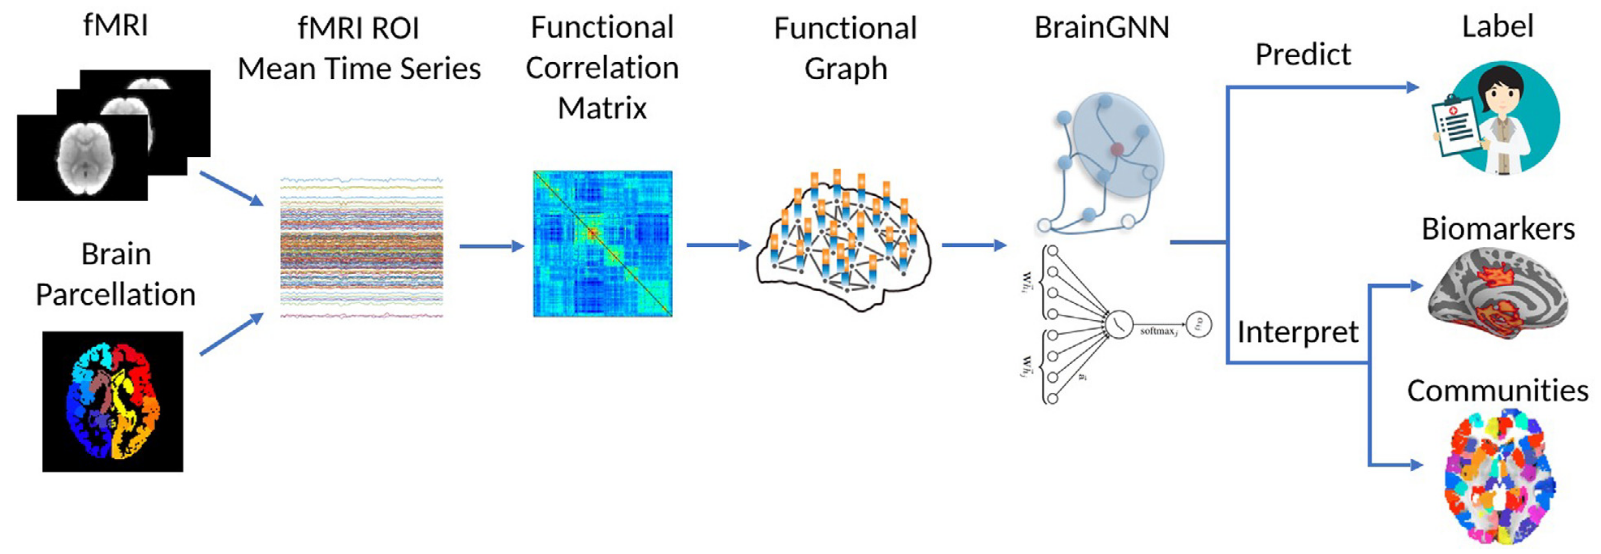
\includegraphics[width=1.0\linewidth]{figures/pipeline.png}
	\caption{Pipeline}
	\cite{LI2021102233}
	\label{fig:pipeline}
\end{figure}


Figure \ref{fig:pipeline} illustrates the implemented experiment pipeline. The whole pipeline starts with a consecutive series of fMRI images. 
fMRI is an imaging technique, which measures blood flow changes. Due to the fact, that blood flow and neural activity are coupled, we can indirectly measure neural activity through fMRI imaging.

In the second step a brain parcellation atlas is used to cluster the brain into $N$ areas. Each cluster is one region of interest (ROI).

For each ROI one time series is constructed. The mean value of the ROI from the first image is the first value of the time series, the mean ROI value of the second image the second time series value and so on. By doing this for all ROIs and all images, a high dimensional time series is received (N = number of clusters from the brain parcellation atlas = number of ROIs = number of time series).

The functional correlation matrix is obtained through calculation of the correlation between all time series.

This matrix can be used as an adjacency matrix for construction of a graph. The column and row index values are the nodes. The cell values are the edge weights. The constructed graph is called functional graph and each node $V = \{v_1, ..., v_N\}$ encodes one ROI (= one brain region) and the edges encode the coupling between the ROIs. The constructed graph is an undirected weighted graph.

To fully describe all features of this graph, two components are needed:
\begin{itemize}
	\item \textbf{Topological structure}: $G = (V, \epsilon)$ defines the topological structure of the graph. $V$ is the set of nodes as one hot encoding and $\epsilon$ is the edge list. The edge list contains two nodes, if they have a connecting edge. The entry $(v_i, v_j)$ encodes a link from node $v_i$ to node $v_j$. Furthermore the weight of each edge is defined by the correlation between the two connected nodes. The edge list can be represented as adjacency matrix $E$ with $e_{ij} = correlation value$ if an edge connects $v_i$ and $v_j$ and $e_{ij} = 0$ if no edge exists between $v_i$ and $v_j$.
	\item \textbf{Node features}: Each node has a feature vector. The node features for a graph can be represented as matrix $H = [h_1, ..., h_N]$ with $h_i$ being the feature vector of node $v_i$.
\end{itemize}

This functional graph is the input to the BrainGNN.

%TODO: was genau ist der Input in das NN
%x = functional correlation matrix -> darauf wird berechnet? x (=vektor) * weights
%edgeindex = edge list -> also adjacency matrix E (in effizienter Form)
%edgeattr = weight einer edge -> also adjacency matrix E (in effizienter Form)
%=> beides genutzt um die Nachbarn zu ermitteln und deren node vectors zu erhalten
%pos = one hot encoding des nodes

The results of the BrainGNN are on the one hand a prediction (e.g. whether a patient is healthy or not) and on the other hand the possibility to interpret the prediction results. BrainGNN makes it possible to detect biomarkers for the prediction tasks and also enables the detection of com\-mu\-nities in the brain.


\subsection{Network architecture}
\label{approach:B}

The network architecture is shown in figure \ref{fig:architecture}. It consists of graph con\-vo\-lu\-tio\-nal layers (Ra-GConv), pooling layers (R-pool) and a Multi Layer Perceptron (MLP). The network consists of two graph neural network (GNN) blocks followed by one MLP. One GNN block consists of one convolutional layer and one pooling layer. The results of these GNN blocks are finally concatenated and passed into a MLP for getting final predictions.

\begin{figure}[ht]
	\centering
	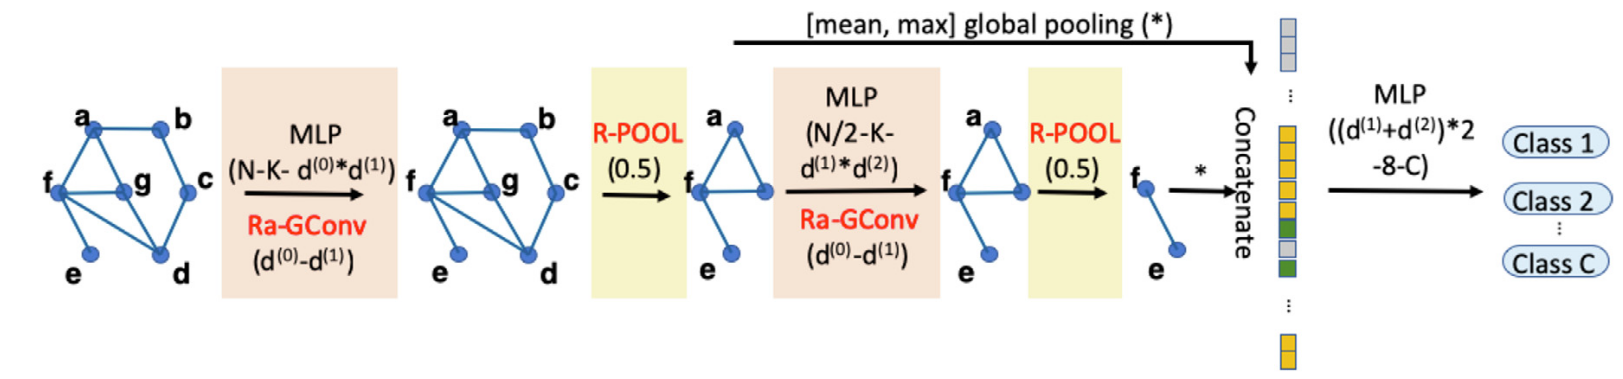
\includegraphics[width=1.0\linewidth]{figures/architecture.png}
	\caption{BrainGNN architecture}
	\cite{LI2021102233}
	\label{fig:architecture}
\end{figure}

\subsubsection{Graph convolutional layer}
\label{approach:Ba}

The node feature vectors of the whole graph are stored in the $H$ matrix. The goal of the convolutional layer is to learn new node feature vectors encoding the topological and semantical information of the graph.

The formula for the forward-pass update of the node feature vectors is defined by Schlichtkrull et al. \cite{10.1007/978-3-319-93417-4_38} as:

\begin{equation}\label{eq:conv_general}
\tilde{h}_i^{(l+1)} = \textrm{relu} \left( W_i^{(l)} h_i^{(l)} + \sum_{j \in \mathcal{N}^{(l)}(i)}^{} e_{ij}^{(l)} W_j^{(l)} h_j^{(l)} \right).
\end{equation}

The superscript $(l)$ denotes the layer and the subscript $i$ denotes the node.
The feature vector of node $i$ in layer $l+1$ is calculated by first multiplying the previous feature vector $h_i^{(l)}$ of node $i$ with the weights $W_i^{(l)}$. Then the feature vectors of all neighbors of node $i$ (neighbor = an edge exists between node $i$ and node $j$) are multiplied with the weights and summed. Up to now the formula is linear. To achieve nonlinearity, the result is passed through an activation function (in this case relu).

%TODO: term oben noch genauer erläutern? was die teilbereiche bedeuten?
%TODO: first iteration on orignal graph -> then on the new representation in following
%TODO: weight normalization

The general idea of the convolutional layer and the novelties of this work are illustrated in figure \ref{fig:convolution}.
\begin{figure}[ht]
	\centering
	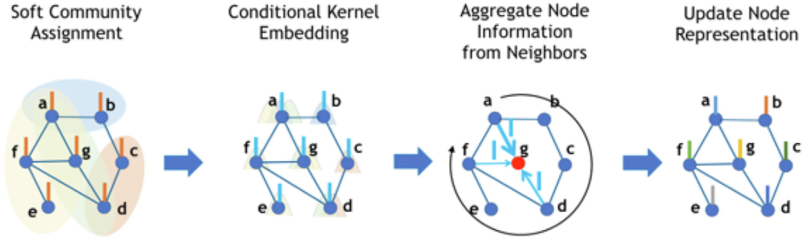
\includegraphics[width=1.0\linewidth]{figures/convolution.png}
	\caption{Graph convolutional layer operations}
	\cite{LI2021102233}
	\label{fig:convolution}
\end{figure}

The two proposed improvements in this work \cite{LI2021102233} for the graph convolutional layer are: 
\begin{enumerate}
	\item Learn different embedding weights for each ROI: \newline
	In eq \ref{eq:conv_general} the weights $W$ are the same for all nodes (ROIs). In this work individual weights are learned for each node. Finally, the vector $\textrm{vec}(W_i^{(l)})$ contains all learned node weights.
	
	The underlying assumption is, that the nodes at the same location but from different graphs are similar. Furthermore, a vector $r_i$ contains the regional information of node $i$ (e.g. the position in the graph). 
	The ordering of all nodes (ROIs) is consistent across different instances. To be able to learn new node feature vectors, which are independent of the ordering method, the regional information $r_i$ is stored as one-hot encoded vector.
	
	As described above the new node feature vector is calculated by ag\-gre\-ga\-ting the neighboring node feature vectors.
	For each node a computation graph of the neighbors is set up. The aggregation of node feature vectors is then done by a neural network with the parameters $\{\Theta_1^{(l)}, \Theta_2^{(l)}\}$ and the input $r_i$.
	
	\begin{equation}\label{eq:conv_1}
	\textrm{vec}(W_i^{(l)}) = f_{MLP}^{(l)}(r_i) = \Theta_2^{(l)} \textrm{relu}(\Theta_1^{(l)} r_i) + b^{(l)}.
	\end{equation}
	
	Eq \ref{eq:conv_1} can be reformulated to:
	\begin{equation}\label{eq:conv_2}
	\textrm{vec}(W_i^{(l)}) = \sum_{u=1}^{K^{(l)}} (\alpha_{iu}^{(l)})^+ \beta_u^{(l)} + b^{(l)}.
	\end{equation}
	
	The weights are decomposed into $\alpha$ (corresponds to $\Theta_1^{(l)}$) and $\beta$ (cor\-re\-sponds to $\Theta_2^{(l)}$). The matrix $\alpha$ contains information about the community membership of nodes. A basis vector for each community is stored in $\beta$.
	
	
	\item Include the edge weight: \newline
	The edge weights in the graph describe the coupling between two nodes. By multiplying node features with the edge weight the connection strength is taken into account.
\end{enumerate}


\subsubsection{Graph pooling layer}
\label{approach:Bb}

The goal of the graph pooling layer is the dimensionality reduction of the graph. Kaiser et al. \cite{doi:10.1073/pnas.1010412107} and Baker et al. \cite{10.1001/jamapsychiatry.2013.3469} have shown, that not all nodes are equally important for predicting neurological disorders. A dimensionality reduction is achieved by keeping the important nodes and removing the other nodes.
The pooling layer is implemented as proposed by Cangea et al. \cite{https://doi.org/10.48550/arxiv.1811.01287} and Gao and Ji \cite{pmlr-v97-gao19a}. For details, please refer to \cite{https://doi.org/10.48550/arxiv.1811.01287} and \cite{pmlr-v97-gao19a}.

The general idea of the pooling layer is illustrated in figure \ref{fig:pooling}. The input are the feature vectors from the convolutional layer. These vectors are then projected onto a learned pooling vector $w^{(l)}$. Based on the difference between the pooling vector and the node feature vectors, a score is calculated. Low scoring nodes are removed, and high scoring nodes are kept.

\begin{figure}[ht]
	\centering
	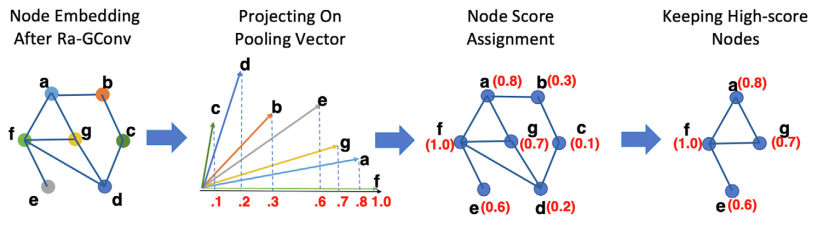
\includegraphics[width=1.0\linewidth]{figures/pooling.png}
	\caption{Graph pooling layer operations}
	\cite{LI2021102233}
	\label{fig:pooling}
\end{figure}

%TODO: Formeln hier aufführen oder weglassen?


%TODO: inwiefern noch auf den Readout layer eingehen?
%TODO: wirklich eigenes Kapitel oder droppen? MLP


\subsection{Training process: loss functions}
\label{approach:C}

As classification loss, the cross entropy loss is used:

\begin{equation}\label{eq:loss_ce}
	L_{ce} = -\frac{1}{M} \sum_{m=1}^{M} \sum_{c=1}^{C} y_{m,c} \log(\hat{y}_{m,c}).
\end{equation}

$M$ denotes the number of instances, $C$ the number of classes, $\hat{y}_{m, c}$ is the model prediction and $y_{m, c}$ is the ground truth label.

To enable interpretability further loss terms are used.
As introduced in section \ref{approach:Bb} a projection from the node representation onto a learned vector $w^{(l)} \in {\mathbb{R}}^{d^{(l)}}$ is used.
The scaling of this vector can vary, but the resulting scores remain the same. 
Consequently, it is not uniquely identifiable, which scores are produced by which learned vectors.
To overcome this issue, a unit loss enforces, that $w^{(l)}$ is a unit vector.

\begin{equation}\label{eq:loss_unit}
L_{unit}^{(l)} = (\| w^{(l)} \|_2 - 1)^2.
\end{equation}

A group-level consistency (GLC) loss is used to ensure, that in the pooling layer, the same nodes are selected across all input instances. This enables the detection of underlying patterns of a disease.
In deeper layers of the network, the graph structure changes. That is why this loss is only used after the first pooling layer, because here the graph structure is still the same as the input graph.

The GLC loss is defined as:

\begin{equation}\label{eq:loss_glc}
L_{GLC} = \sum_{c=1}^{C} \sum_{m,n \in \mathcal{I}_c}^{} \| \tilde{s}_m^{(1)} - \tilde{s}_n^{(1)} \|^2 = 2 \sum_{c=1}^{C} Tr((S_c^{(1)})^T L_c S_c^{(1)}).
\end{equation}

It calculates the pooling score similarity between two instances $m$ and $n$ ($\| \tilde{s}_m^{(1)} - \tilde{s}_n^{(1)} \|^2$). By taking the sum over all classes $C$ (first sum) and the sum over all instances $M$ in one batch (second sum), the pairwise pooling score similarities are calculated between all instances.
%By minimizing this GLC loss term, it is ensured, that the scores of the instances are similar and therefore the selection of nodes for removing or keeping is similar.
%If the scores of two instances are similar, the GLC loss is low.
The way how this is calculated is expressed on the right hand side of the equation. For details about this, please refer to \cite{LI2021102233}.

The TopK pooling loss makes sure, that the nodes which are removed have a significantly different score compared to the nodes which are not removed. 
First of all, the scores are passed through a sigmoid layer. After this, the score values are in the range between 0 and 1. These scores are then sorted in descending order for all $M$ instances. Finally, a constraint is applied to the ordering for all $M$ instances, which leads to a more dispersed distribution. 
Mathematically, it is formulated as binary cross-entropy:

\begin{equation}\label{eq:loss_tpk}
L_{TPK}^{(l)} = - \frac{1}{M} \sum_{m=1}^{M} \frac{1}{N^{(l)}} \left(\sum_{i=1}^{k} \log(\hat{s}_{m, i}^{(l)}) + \sum_{i=1}^{N^{(l)}-k} \log (1- \hat{s}_{m, i+k}^{(l)})\right).
\end{equation}

All presented loss functions above are part of the final loss function (with $\lambda_1$ and $\lambda_2$ as hyperparameters):

\begin{equation}\label{eq:loss_total}
L_{total} = L_{ce} + \sum_{l=1}^{L} L_{unit}^{(l)} + \lambda_1 \sum_{l=1}^{L} L_{TPK}^{(l)} + \lambda_2 L_{GLC}.
\end{equation}
